\documentclass[]{article}
\usepackage{lmodern}
\usepackage{amssymb,amsmath}
\usepackage{ifxetex,ifluatex}
\usepackage{fixltx2e} % provides \textsubscript
\ifnum 0\ifxetex 1\fi\ifluatex 1\fi=0 % if pdftex
  \usepackage[T1]{fontenc}
  \usepackage[utf8]{inputenc}
\else % if luatex or xelatex
  \ifxetex
    \usepackage{mathspec}
  \else
    \usepackage{fontspec}
  \fi
  \defaultfontfeatures{Ligatures=TeX,Scale=MatchLowercase}
\fi
% use upquote if available, for straight quotes in verbatim environments
\IfFileExists{upquote.sty}{\usepackage{upquote}}{}
% use microtype if available
\IfFileExists{microtype.sty}{%
\usepackage{microtype}
\UseMicrotypeSet[protrusion]{basicmath} % disable protrusion for tt fonts
}{}
\usepackage[margin=1in]{geometry}
\usepackage{hyperref}
\hypersetup{unicode=true,
            pdftitle={Salad with a Side of Plastic: Comparing Microplastic Pollution in Romaine Lettuce Sold with or without Plastic Packaging},
            pdfauthor={Bailey Lai},
            pdfborder={0 0 0},
            breaklinks=true}
\urlstyle{same}  % don't use monospace font for urls
\usepackage{longtable,booktabs}
\usepackage{graphicx,grffile}
\makeatletter
\def\maxwidth{\ifdim\Gin@nat@width>\linewidth\linewidth\else\Gin@nat@width\fi}
\def\maxheight{\ifdim\Gin@nat@height>\textheight\textheight\else\Gin@nat@height\fi}
\makeatother
% Scale images if necessary, so that they will not overflow the page
% margins by default, and it is still possible to overwrite the defaults
% using explicit options in \includegraphics[width, height, ...]{}
\setkeys{Gin}{width=\maxwidth,height=\maxheight,keepaspectratio}
\IfFileExists{parskip.sty}{%
\usepackage{parskip}
}{% else
\setlength{\parindent}{0pt}
\setlength{\parskip}{6pt plus 2pt minus 1pt}
}
\setlength{\emergencystretch}{3em}  % prevent overfull lines
\providecommand{\tightlist}{%
  \setlength{\itemsep}{0pt}\setlength{\parskip}{0pt}}
\setcounter{secnumdepth}{0}
% Redefines (sub)paragraphs to behave more like sections
\ifx\paragraph\undefined\else
\let\oldparagraph\paragraph
\renewcommand{\paragraph}[1]{\oldparagraph{#1}\mbox{}}
\fi
\ifx\subparagraph\undefined\else
\let\oldsubparagraph\subparagraph
\renewcommand{\subparagraph}[1]{\oldsubparagraph{#1}\mbox{}}
\fi

%%% Use protect on footnotes to avoid problems with footnotes in titles
\let\rmarkdownfootnote\footnote%
\def\footnote{\protect\rmarkdownfootnote}

%%% Change title format to be more compact
\usepackage{titling}

% Create subtitle command for use in maketitle
\providecommand{\subtitle}[1]{
  \posttitle{
    \begin{center}\large#1\end{center}
    }
}

\setlength{\droptitle}{-2em}

  \title{Salad with a Side of Plastic: Comparing Microplastic Pollution in
Romaine Lettuce Sold with or without Plastic Packaging}
    \pretitle{\vspace{\droptitle}\centering\huge}
  \posttitle{\par}
    \author{Bailey Lai}
    \preauthor{\centering\large\emph}
  \postauthor{\par}
      \predate{\centering\large\emph}
  \postdate{\par}
    \date{2019 May 09}


\begin{document}
\maketitle

\hypertarget{abstract}{%
\subsubsection{Abstract}\label{abstract}}

Microplastic contamination, resulting from the breaking down of larger
plastic waste, covers vast swathes of the Earth, and its worldwide
proliferation has worrying implications for worldwide human health.
There is a growing body of research indicating humans are consuming
microplastics through a variety of foods, leading to microplastic
bioaccumulation that can cause harm to humans. However, most studies
have focused on the risk of consuming seafood contaminated with
microplastics, especially filtering bivalves. This research aims to
investigate microplastic levels in romaine lettuce commercially sold in
grocery stores around Claremont, California, investigating whether
plastic packaging of pre-washed produce has higher potential for
microplastic contamination versus unwashed unpackaged produce. In
comparing packaged and unpackaged lettuce, the null hypothesis of
``there is no difference in microplastic quantities in romaine lettuce
with or without plastic packaging'' could not be rejected (parametric
test p-value = 0.38; non-parametric test p-value = 0.58). This brings
into consideration whether our study can broaden our focus to
encapsulate produce exposure to airborne microplastics, the extent of
laboratory microplastic contamination and the future of research into
the prevalence of microplastics in the larger environment.

\hypertarget{introduction}{%
\subsubsection{Introduction}\label{introduction}}

Microplastic, generally defined as any small fragments of plastic
between 10 micrometers and five millimeters in diameter, presents a
major environmental pollution dilemma. The prevalence of plastic in
modern society and the inability of most plastic particles, polymers,
and fibers to naturally biodegrade mean huge amounts of plastic waste
have accumulated across all corners of the globe and through all forms
of human products (GESAMP 2016; Andrady 2017). Wherever microplastics
end up, they accumulate in biota, some of which ends up consumed by
humans. The long-term effects of microplastics in humans are not fully
understood, but plastic additives and its bonds with toxic materials can
potentially cause adverse health effects for humans. Despite this, there
is still much research to be done on microplastics found in consumed
foods aside from seafood, such as in produce. This study aims to
determine whether commercially-sold produce wrapped in plastic
packaging, such as pre-washed romaine lettuce, changes the amount of
microplastic deposited on its surface (and therefore consumed) as
opposed to produce sold without packaging.

Most existing microplastic research focuses on microplastic accumulated
in marine life and commercially-sold seafood like bivalves (Cauwenberghe
and Jannsen 2014). This means there has been a surprising lack of
research on terrestrial microplastic bioaccumulation in the past (Rillig
2012). Though plastics can break down into smaller sizes, plastic
polymers do not easily break down at the microscopic and molecular level
(Liboiron 2015). The toxic materials that bond with plastics at the
microscopic level ultimately make microplastics such a pressing health
issue for plants, animals, humans, and other living organisms (Liboiron
2015). des Rieux et al. (2005) found that ingested nanoparticles can
affect transcellular transport using in vitro models of follicle
associated epthelium (FAE) in the human intestine, with amine
nanoparticles (consisting of a nitrogen atom and lone pair) transported
more easily than carboxyl nanoparticles (containing the atoms COOH),
suggesting functional groups of plastic nanoparticle compounds play a
role in absorption through the intestines. In addition, other studies
have shown common plastic additives like phthalates and Bisphenol A
(BPA) can affect the hormone systems of different organisms (Machado et
al.~2017). Because most microplastics research is in the past decade,
there is no scientific consensus on how significant long-term and
continuous ingestion of microplastics in food is when compared to
overall microplastic exposure. By investigating produce at the stage of
production nearest to consumption (in the grocery store), this research
aims to begin to create a more robust understanding of how all foodways
impact human microplastic exposure, and how processing tactics, such as
packaging, play a role in exposure.

Multiple overarching questions are therefore developed to conduct this
research. Are microplastics found in romaine lettuce intended for human
consumption? If yes, do microplastic concentrations vary depending on
whether or not they were sold in plastic packaging at the point of
purchase? Because of romaine lettuce's availability both in unpackaged
heads and prepared plastic bags, it serves as the ideal produce through
which to investigate how the phenomenon of how packaging impacts
microplastic exposure and subsequent leaching. Furthermore, this
research will be conducted using a hypothesis test, where a null
hypothesis will be rejected or not rejected based on whether a p-value
of \textless{} 0.05 is obtained. For the purpose of this research, the
null hypothesis is ``there is no difference in microplastic quantities
in romaine lettuce sold with or without plastic packaging.'' Our
alternative hypothesis is that there is a statistically significant
difference in microplastic counts from romaine lettuce sold with plastic
packaging versus romaine lettuce sold without. This metric will be used
to assess the impact of plastic packaging on microplastic in
commercially-sold produce.

By conducting this study, we hope to better understand the exposure to
microplastics in situations aside from eating seafood and marine life.
The prevalence of plastics in today's world means microplastics are
found and inevitably ingested by humans on a daily basis. What
microplastic ingestion means for the long-term health effects on humans
is not yet fully understood, but we do know that plastics in general can
leach harmful chemicals and also can attract toxic chemicals onto its
surface. Studying the presence of microplastics in a commonly packaged
grocery item like romaine lettuce can give us more insight to how
plastics get into our digestive systems and perhaps lead us to solutions
for reducing plastic contamination in our everyday lives.

\hypertarget{methods}{%
\subsubsection{Methods}\label{methods}}

The following methods are based off of prior established methods for
obtaining microplastic counts from food products (Löder et al.~2017,
Maes et al.~2017, Karlsson et al.~2017, and Quinn et al.~2018).

We purchased two unpackaged heads of romaine lettuce and two bags of
romaine lettuce in plastic packaging from each of the chosen five stores
in the cities of Claremont and Pomona. We chose only stores that sell
both unpackaged heads AND packaged lettuce (lettuce packaged as chopped
salad is acceptable). This led us to select the following supermarkets:
Sprouts on Foothill Blvd, Stater Bros.~on N Garey Ave, Cardenas on E
Holt Ave, El Super on E Holt Ave, and Super King on Auto Center Dr.~We
put the unpackaged romaine lettuce into paper bags to minimize
contamination during transit.

In the lab, we used a glass blender to homogenize the lettuce with
water. All equipment in contact with lettuce were first thoroughly
washed with Milli-Q deionized water for each successive sample. For each
sample of unbagged lettuce, we washed the head in Milli-Q deionized
water, then tore out leaves and inserted them into the blender until it
reached the top. Bagged lettuce was not washed, since they are labeled
``pre-washed'' and we wanted to test the difference. Bagged lettuce was
poured straight from the bag into the blender until it reached the top.
Afterwards, we poured in 200 mL of Milli-Q deionized water into the
blender. We blended the mix of lettuce and water for 30 seconds under
the slower ``stir/grind'' setting, then 60 seconds under the faster
``cream/fruit smoothie'' setting. We strained the homogenized lettuce
and water through a 5 mm stainless steel sieve into a glass beaker to
obtain 100 mL of solution. This process was repeated for each sample,
for a total of 20 experimental samples (two unbagged, two bagged from
each of the five stores).

To break down the cellulose in the lettuce solution, we added 5 mL
cellulase from \emph{Aspergillus niger} to separate particles in the
solution by density, and then we added 10 mL phosphate-buffered saline
(PBS) to each beaker. 1 L of phosphate-buffered saline solution was
prepared using 8 g sodium chloride (NaCl), 200 mg potassium chloride
(KCl), 1.44 g disodium phosphate
(Na\textsubscript{2}HPO\textsubscript{4}), and 240 mg monopotassium
phosphate (KH\textsubscript{2}PO\textsubscript{4}) prepared in deionized
water, then set to pH 5 using hydrochloric acid (HCl). Three blank
control samples were prepared using 100 mL Milli-Q deionized water in a
glass beaker. The beakers were then covered with aluminium foil wrap and
incubated at 50°C for four days.

After incubation, we added 50 mL NaCl solution to each beaker (density =
1.2 g NaCl / 1 mL water, 1440 mL solution stirred in 2 L volumetric
flask for 10 minutes). For each beaker, 5 mL of 0.08 g/mL Red Nile dye
solution was added and allowed to stain the sample solution for 30
minutes. For each of the 23 total samples, 40 mL of solution was
extracted from the top of the beaker using a glass vacuum and glass
pipette through a sheet of filter paper. The filter paper was placed in
glass containers and covered with aluminium foil to let dry overnight.
We then used a digital microscope with fluorescent light (red
fluorescent 100\% brightness, 110 ms capture) to count stained
microplastic particles next to four randomly generated points at 4X zoom
for each sample of filter paper (Figure 1). Four microplastic counts
were obtained for each of the 20 experimental samples and 3 blank
samples.

\begin{figure}
\centering
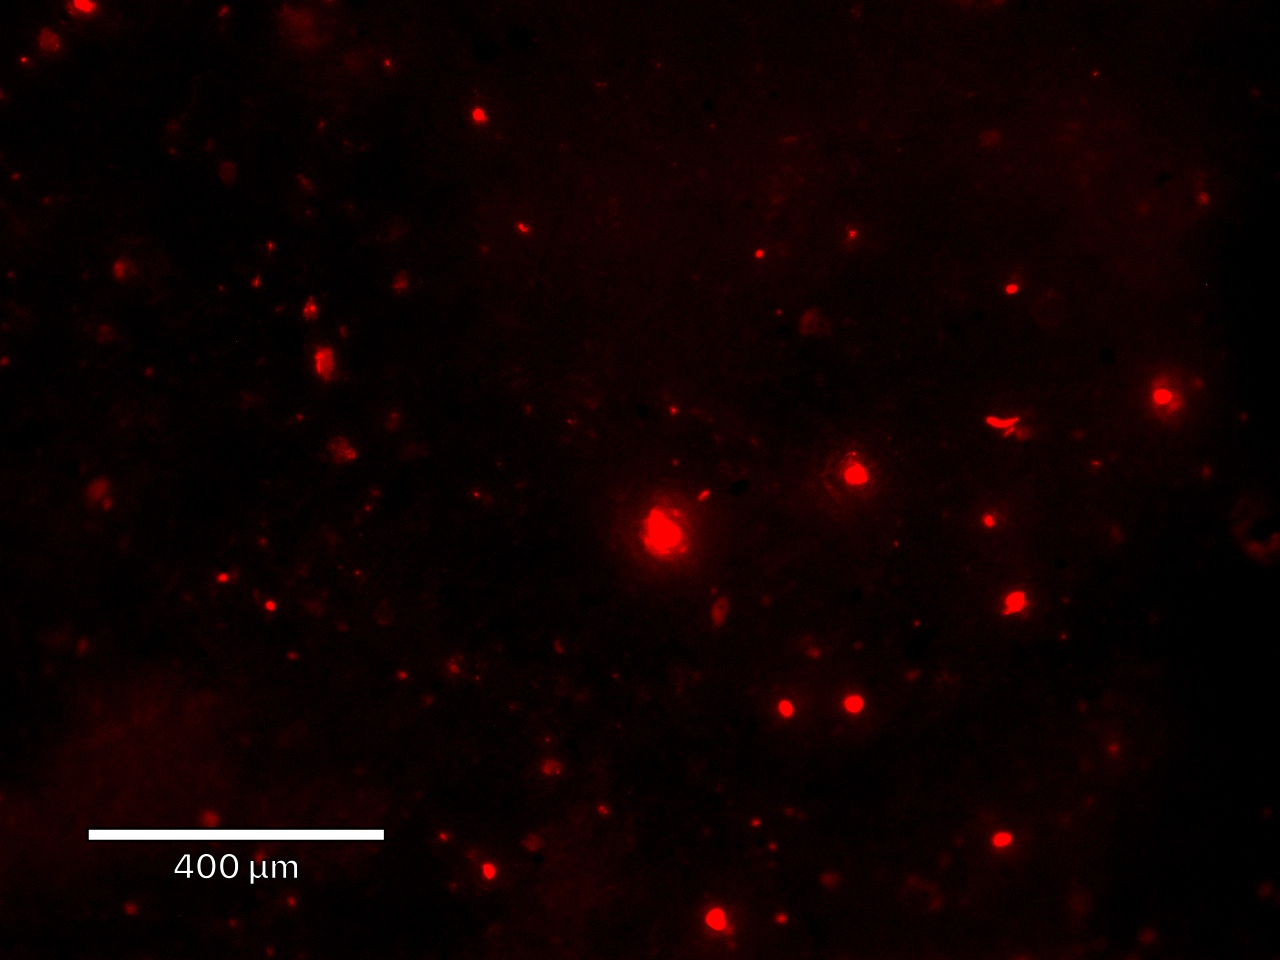
\includegraphics{Sprouts_UB_2_Image_0001.jpg}
\caption{\emph{\textbf{Figure 1.} The image captured by the Revolve
digital microscope for Sprouts Unbagged Sample \#2, point 1.}}
\end{figure}

Statistical analysis was conducted using the program R (R Core Team
2019). In the analysis, we calculated the average of the eight unbagged
counts and the average of the eight bagged counts for each of the five
stores, giving us five bagged averages and five unbagged averages. We
compared each store's bagged versus unbagged average with the parametric
paired t-test (for normal distribution) and nonparametric paired
Wilcoxon signed-rank test (for non-normal distribution), obtaining one
p-value for each of the two tests.

\hypertarget{results}{%
\subsubsection{Results}\label{results}}

\includegraphics{microplastics_FINAL_DRAFT_files/figure-latex/graphs for all lettuce data-1.pdf}

\emph{\textbf{Figure 1.} Boxplot of Microplastic Counts}

\includegraphics{microplastics_FINAL_DRAFT_files/figure-latex/qqplot for UB-1.pdf}

\emph{\textbf{Figure 2.} Normal Q-Q Plot of Unbagged Lettuce}

\includegraphics{microplastics_FINAL_DRAFT_files/figure-latex/qqplot for BG-1.pdf}

\emph{\textbf{Figure 3.} Normal Q-Q Plot of Bagged Lettuce}

\begin{longtable}[]{@{}lll@{}}
\toprule
Type & Average Count & Net Experimental Count\tabularnewline
\midrule
\endhead
Unbagged & 32.775 & 8.025\tabularnewline
Bagged & 39.700 & 14.950\tabularnewline
Blank & 24.750 & -\tabularnewline
\bottomrule
\end{longtable}

\emph{\textbf{Table 1.} Average Microplastic Count in Grocery-Bought
Romaine Lettuce}

\begin{longtable}[]{@{}lll@{}}
\toprule
Test & p-value & Statistical significance?\tabularnewline
\midrule
\endhead
1. paired t-test & 0.38 & no\tabularnewline
2. Wilcoxon signed-rank test & 0.58 & no\tabularnewline
\bottomrule
\end{longtable}

\emph{\textbf{Table 2.} Test of differences between bagged and unbagged
microplastic counts paired with each store}

We did both the parametric and non-parametric paired tests because the
unbagged and bagged samples had different distributions (Figures 1-3).
The Shapiro-Wilk normality test for the bagged lettuce indicated normal
distribution (W = 0.77, p-value = 0.045), whereas the Shapiro-Wilk
normality test for the unbagged lettuce indicated non-normal
distribution (W = 0.87, p-value = 0.28). We do not reject the null
hypothesis based on the lack of statistical significance in the paired
t-test (p-value = 0.38) and Wilcoxon signed-rank test (p-value = 0.58).
This indicates there is no significant difference in microplastic count
between unbagged heads of romaine lettuce and romaine lettuce bagged in
plastic packaging (Table 2).

\hypertarget{discussion}{%
\subsubsection{Discussion}\label{discussion}}

The high p-value in both the non-parametric test and parametric test
indicates the difference between the bagged and unbagged microplastic
counts are not statistically significant. One possible reason is the
amount of microplastics deposited in produce wrapped in plastic
packaging may be comparable to the amount deposited on unbagged produce
in transit and processing as airborne plastic dust. Bagged lettuce may
be exposed to high amounts of microplastic in the processing plant, but
is washed prior to being air-sealed until consumption. Unbagged lettuce,
on the other hand, is exposed to any outside dust pollution that settles
on its surface from the processing facility to the grocery aisle and the
trip from the supermarket to the consumer's kitchen. Microplastics can
be introduced to any time in the production and transportation of
produce, all the way up to consumption.

Most food bought in groceries and stores today go through many
manufacturing processes and machinery, putting products into contact
with plastic residue and potential contaminants.Considering the
probability of airborne microplastics cross-contaminating controlled
indoor lab experiments, commercially-available produce harvested \&
processed by plastic machinery and/or sold in wrapped plastics will
likely contain microplastic as well (Machado et al.~2017). Multiple
studies have shown commercial food products like honey, table salt, beer
contain trace amounts of microplastic fibers (Karami et al.~2017,
Iñiguez et al.~2017, Liebezeit and Liebezeit 2013, 2014). One study has
shown that microplastics can be found in agricultural fields that use
fertilizer from human wastewater systems (Machado et al 2017). This
raises the question of whether comparing bagged and unbagged produce is
appropriate, or if future research should explore microplastic
consumption in a larger context of surrounding microplastic in existing
agricultural practices and built environments.

No investigation into microplastics in produce has been conducted
before, making the process of creating procedures difficult. However, in
the non-seafood studies evaluated, microplastic quantities were between
1-660 microplastics per kilogram of substance. As with all
investigations into microplastics in foods, there is significant risk of
sample contamination, which may explain the extreme variation in
numbers. Additionally, three of the four studies found minimus of 16-50
microplastics per kilogram, and maximums of 254-660 microplastics per
kilogram, fairly comparable numbers when contamination and random
variation is considered. The microplastics found in romaine lettuce
heads may fall within these boundaries (Karami et al.~2017, Iñiguez et
al.~2017 Liebezeit and Liebezeit 2013, 2014). However, as with most
microplastic studies, some potential confounding factors do exist.

Our methodology may also impacted the final counts. One issue arose with
the way in which we obtained the sample solution. When we used a sieve
to filter the blended lettuce water, most of the visible fibre solids
congealed atop the sieve, potentially filtering out microplastics among
the lettuce from the resulting solution we tested. Contamination of
samples is a major concern, via airborne particulates, plastics which
may remain in deionized water, and the presence of plastics (clothing,
equipment, etc) in the lab. Another issue we ran into was how to
quantify dyed particles. Though most particles appeared circular and
artificial and most likely microplastic, it was hard to assess whether
some dyed material were plastic or lettuce fibres and strands. If time
permits, future studies can look into digesting more of the lettuce
fibres with the multi-week enzymatic digestions described in Löder et
al. (2017), rather than separating most of the solids with a sieve and
using one enzymatic digestion. This may provide a more encompassing and
accurate microplastic count.

\hypertarget{conclusion}{%
\subsubsection{Conclusion}\label{conclusion}}

Our study did not find a statistically significant difference in
microplastic counts between romaine lettuce sold pre-washed in plastic
packaging versus romaine lettuce sold unpackaged. Though our study did
not have conclusive findings, future microplastics research is highly
needed based on the little literature we found on microplastics in
produce and in terrestrial environments. The fact that we counted
microplastics in all our samples, even in the blanks, suggests
microplastics are omnipresent in our lives. This reality underscores the
necessity, discussed by Rist et al. (2018), of expanding and
contextualizing the debate around microplastics. After all, food
consumption is still just one of many possible ways in which we can get
exposed to microplastic pollution every day. The larger implications of
airborne microplastics within produce facilities or carried around the
atmosphere by wind, as well as the processes of microplastic
accumulation in agricultural fields and other land-based ecosystems
should be better understood to best grapple with increasing plastics in
our world.

\hypertarget{works-cited}{%
\subsubsection{Works Cited}\label{works-cited}}

Andrady, AL. 2017. The plastic in microplastics: a review. Mar Pollut
Bull {[}Internet{]}. {[}published 2017 Jan 30; cited 2019 Mar 30{]};
119: 12-22.

Claessens M, Van Cauwenberghe L, Vandegehuchte MB, Janssen CR. 2013. New
techniques for the detection of microplastics in sediments and field
collected organisms. Mar Pollut Bul {[}Internet{]}. {[}published 2013
May 15; cited 2019 Mar 31{]}; 70(1-2): 227-233.

des Rieux A, Ragnarsson EG, Gullberg E, Préat V, Schneider YJ, Artursson
P. 2005. Transport of nanoparticles across an in vitro model of the
human intestinal follicle associated epithelium. Eur J Pharm Sci
{[}Internet{]}. {[}cited 2019 Apr 08{]}; 25(4-5): 455-465.

{[}GESAMP{]} Joint Group of Experts on the Scientific Aspects of Marine
Environmental Protection. 2016. Sources, Fate And Effects Of
Microplastics In The Marine Environment: Part Two Of A Global
Assessment. GESAMP {[}Internet{]}. {[}cited 2019 Apr 08{]}; 93:1-220.

Iñiguez M, Conesa J, Fullana A. 2017. Microplastics in Spanish Table
Salt. Scientific Reports {[}Internet{]}. {[}cited 2019 Apr 08{]};
7:8620.

Karami A, Golieskardi A, Choo C, Larat V, Galloway T, Salamatinia B.
2017. The presence of microplastics in commercial salts from different
countries. Nature Scientific Articles {[}Internet{]}. {[}cited 2019 Apr
08{]}; 7: 46173.

Karlsson T, Vethaak A, Almrothd B, Ariese F, van Velzen M, Hassellöv M,
Leslie H. 2017. Screening for microplastics in sediment, water, marine
invertebrates and fish: Method development and microplastic
accumulation. Mar Pollut Bul {[}Internet{]}. {[}cited 2019 Apr 08{]};
122:403-408.

Kühn S, Rebolledo ELB, Van Franeker JA. 2015. Deleterious effects of
litter on marine life. Mar Anthro Litter {[}Internet{]}. {[}cited 2019
Apr 08{]}; 75--116.

Liboiron M. 2016. Redefining pollution and action: the matter of
plastics. J Material Cult {[}Internet{]}. {[}cited 2019 Mar 30{]};
21(1): 87-110.

Liebezeit G, Liebezeit E. 2013. Non-pollen particulates in honey and
sugar. Food Additives \& Contaminants: Part A {[}Internet{]}. {[}cited
2019 Mar 30{]}; 30(12):2136-2140.

Liebezeit G, Liebezeit E. 2014. Synthetic particles as contaminants in
German beer. Food Additives \& Contaminants: Part A {[}Internet{]}.
{[}cited 2019 Mar 30{]}; 31(9):1574-1578.

Löder M, Imhof H, Ladehoff M, Löschel L, Lorenz C, Mintenig S, Piehl S,
Primpke S, Schrank I, Laforsch C, Gerdts G. 2017. Enzymatic Purification
of Microplastics in Environmental Samples. Enviro Sci Technol
{[}Internet{]}. {[}cited 2019 Mar 30{]}; 51:14283-14292.

Maes T, Jessop R, Wellner N, Haupt K, Mayes A. 2017. A rapid-screening
approach to detect and quantify microplastics based on fluorescent
tagging with Nile Red. Sci Reports {[}Internet{]}. {[}cited 2019 Apr
08{]}; 7:44501.

Machado AAS, Kloas W, Zarfl C, Hempel S, Rillig MC. 2017. Microplastics
as an emerging threat to terrestrial ecosystems. Glob Change Biol
{[}Internet{]}. {[}published 2017 December 15; cited 2019 March 31{]};
24(4): 1405-1416.

R Core Team. 2019. R: A language and environment for statistical
computing. R Foundation for Statistical Computing {[}Internet{]}.
\url{http://www.R-project.org/}.

Rillig MC. 2012. Microplastic in terrestrial ecosystems and the soil?
Environ Sci Technol {[}Internet{]}. {[}published 2012 May 31; cited 2019
April 01{]} 46: 6453-6454.

Quinn B, Murphy F, Ewins. 2017. Validation of density separation for the
rapid recovery of microplastics from sediment. Anal Methods
{[}Internet{]}. {[}cited 2019 Apr 01{]}; 9(9):1491-1498.


\end{document}
